
















































































































































































































%definizione colori per tabelle (tranne copertina)
\definecolor{redafk}{RGB}{255, 71, 87}
\definecolor{grey2}{RGB}{204, 204, 204}
\definecolor{lastrowcolor}{RGB}{156, 198, 214}
\definecolor{greyRowafk}{RGB}{234, 234, 234}
\rowcolors{2}{grey2}{greyRowafk}
\renewcommand{\arraystretch}{1.5}

\subsection{Fase di Validazione e collaudo}
\subsubsection{Distribuzione oraria}
In questa fase i ruoli sono così suddivisi:

%tabella ore
\begin{table}[H]
\centering\renewcommand{\arraystretch}{1.5}
\caption{Validazione e Collaudo}
\vspace{0.2cm}
\begin{tabular}{ c | c | c | c | c | c | c | c }
\rowcolor{redafk}
\textcolor{white}{\textbf{Nominativo}} & \textcolor{white}{\textbf{Re}} & 
\textcolor{white}{\textbf{Am}} & \textcolor{white}{\textbf{An}} &
\textcolor{white}{\textbf{Pt}} & \textcolor{white}{\textbf{Pm}} &
\textcolor{white}{\textbf{Ve}} & \textcolor{white}{\textbf{Totale}} \\
Simone Federico Bergamin 	& 5 	& - 	& - 	& - 	& 8 	& 12 	& 25 \\
Alessandro Canesso 			& 4 	& 4 	& - 	& - 	& - 	& 15 	& 23 \\
Victor Dutca 				& 5 	& - 	& - 	& - 	& 5 	& 15 	& 25 \\
Fouad Farid					& - 	& 6 	& - 	& - 	& 7 	& 12 	& 25 \\
Simone Meneghin 			& - 	& 9 	& - 	& - 	& - 	& 16 	& 25 \\
Olivier Utshudi 			& - 	& 4 	& - 	& 4 	& 5 	& 12 	& 25 \\
Davide Zilio 				& 6 	& - 	& - 	& 8 	& - 	& 11 	& 25 \\
\rowcolor{lastrowcolor}
\textbf{Ore totali ruolo} & \textbf{20} & \textbf{23} & \textbf{0} & \textbf{12} & \textbf{25} & \textbf{93} & \textbf{173} \\
\end{tabular}
\end{table}

I dati ottenuti sono riassunti nel seguente istogramma: 
\begin{figure}[H]
\centering
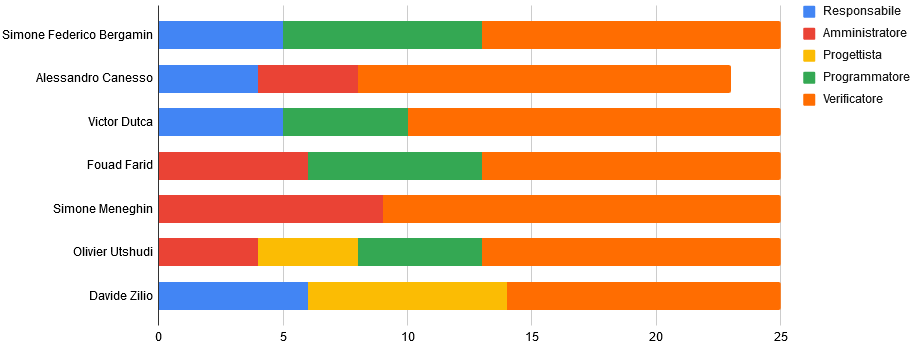
\includegraphics[scale=0.60]{img/grafici/tabella_fase_val_col.png}
\caption{Istogramma della ripartizione delle ore per ruolo nella fase di Validazione e collaudo}
\end{figure}

\subsubsection{Prospetto economico}
In questa fase il costo per ogni ruolo è il seguente:

%tabella costi
\begin{table}[H]
\centering\renewcommand{\arraystretch}{1.5}
\caption{Prospetto dei costi nella fase di Validazione e collaudo}
\vspace{0.2cm}
\begin{tabular}{ c | c | c  }
\rowcolor{redafk}
\textcolor{white}{\textbf{Ruolo}} & \textcolor{white}{\textbf{Ore}} & 
\textcolor{white}{\textbf{Costo}}  \\
Responsabile & 20 & 600€ \\
Amministratore & 23 & 460€ \\
Analista & - & - \\
Progettista	& 12 & 264€ \\
Programmatore & 25 & 375€  \\
Verificatore & 93 & 1395€  \\
\rowcolor{lastrowcolor}
\textbf{Totale} & \textbf{173} & \textbf{3094€}  \\
\end{tabular}
\end{table}

I dati ottenuti si possono riassumere nel seguente areogramma:
\begin{figure}[H]
\centering
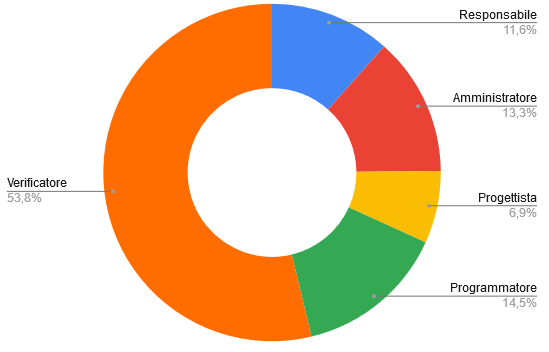
\includegraphics[scale=0.60]{img/grafici/torta_fase_val_col.png}
\caption{Areogramma della ripartizione dei costi per ruolo nella fase di Validazione e collaudo}
\end{figure}


\subsection{Riepilogo}
\subsubsection{Ore rendicontate con investimento}
\paragraph{Distribuzione oraria} \mbox{} \\ \mbox{} \\
Vengono riportate il totale delle ore del progetto in cui sono presenti le ore di investimento e le
ore rendicontate a carico del committente:

%tabella ore
\begin{table}[H]
\centering\renewcommand{\arraystretch}{1.5}
\caption{Distribuzione totale delle ore dell'intero progetto con investimento}
\vspace{0.2cm}
\begin{tabular}{ c | c | c | c | c | c | c | c }
\rowcolor{redafk}
\textcolor{white}{\textbf{Nominativo}} & \textcolor{white}{\textbf{Re}} & 
\textcolor{white}{\textbf{Am}} & \textcolor{white}{\textbf{An}} &
\textcolor{white}{\textbf{Pt}} & \textcolor{white}{\textbf{Pm}} &
\textcolor{white}{\textbf{Ve}} & \textcolor{white}{\textbf{Totale}} \\
Simone Federico Bergamin 	& 11 	& 13 	& 30 	& 19 	& 31 	& 41 	& 145 \\
Alessandro Canesso 			& 16 	& 18 	& 16 	& 20 	& 27 	& 46 	& 143 \\
Victor Dutca 				& 17	& 14 	& 19 	& 20 	& 32 	& 41 	& 143 \\
Fouad Farid					& 11	& 18 	& 12 	& 32 	& 27 	& 43 	& 143 \\
Simone Meneghin 			& 8 	& 17 	& 23 	& 32 	& 29 	& 40 	& 149 \\
Olivier Utshudi 			& 8 	& 16 	& 13 	& 30 	& 32 	& 49 	& 148 \\
Davide Zilio 				& 13 	& 11 	& 30 	& 18 	& 20 	& 51 	& 143 \\
\rowcolor{lastrowcolor}
\textbf{Ore totali ruolo} & \textbf{84} & \textbf{107} & \textbf{143} & \textbf{171} & \textbf{198} & \textbf{311} & \textbf{1014} \\
\end{tabular}
\end{table}

Una rappresentazione visiva della suddivisione oraria viene data dal seguente grafico:
\begin{figure}[H]
\centering
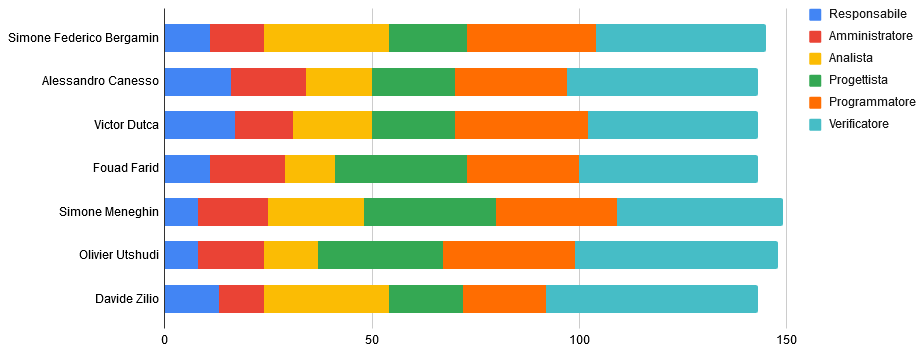
\includegraphics[scale=0.60]{img/grafici/tabella_tot_con_analisi.png}
\caption{Istogramma della ripartizione delle ore totali per ruolo con investimento}
\end{figure}

\paragraph{Prospetto economico} \mbox{} \\ \mbox{} \\
Il costo totale con investimento è riportato nella seguente tabella:

%tabella costi
\begin{table}[H]
\centering\renewcommand{\arraystretch}{1.5}
\caption{Costi totali con investimento}
\vspace{0.2cm}
\begin{tabular}{ c | c | c  }
\rowcolor{redafk}
\textcolor{white}{\textbf{Ruolo}} & \textcolor{white}{\textbf{Ore}} & 
\textcolor{white}{\textbf{Costo}}  \\
Responsabile & 84 & 2520€ \\
Amministratore & 107 & 2140€ \\
Analista & 143 & 3575€ \\
Progettista	& 171 & 3762€ \\
Programmatore & 198 & 2970€  \\
Verificatore & 311 & 4665€  \\
\rowcolor{lastrowcolor}
\textbf{Totale} & \textbf{1014} & \textbf{19632€}  \\
\end{tabular}
\end{table}

I dati ottenuti si possono riassumere nel seguente areogramma:
\begin{figure}[H]
\centering
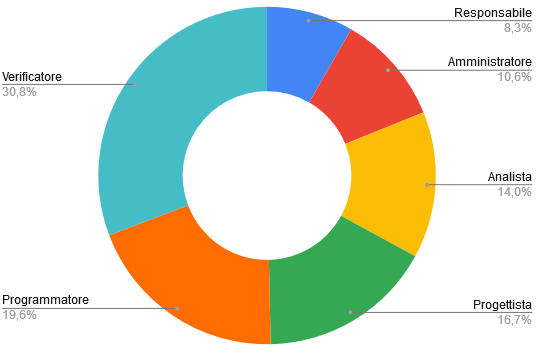
\includegraphics[scale=0.60]{img/grafici/torta_tot_con_analisi.png}
\caption{Areogramma della ripartizione dei costi totali per ruolo con investimento}
\end{figure}

\subsubsection{Ore rendicontate senza investimento}
\paragraph{Distribuzione oraria} \mbox{} \\ \mbox{} \\
Le ore rendicontate sono riassunte nella seguente tabella:

%tabella ore
\begin{table}[H]
\centering\renewcommand{\arraystretch}{1.5}
\caption{Distribuzione totale delle ore dell'intero progetto senza investimento}
\vspace{0.2cm}
\begin{tabular}{ c | c | c | c | c | c | c | c }
\rowcolor{redafk}
\textcolor{white}{\textbf{Nominativo}} & \textcolor{white}{\textbf{Re}} & 
\textcolor{white}{\textbf{Am}} & \textcolor{white}{\textbf{An}} &
\textcolor{white}{\textbf{Pt}} & \textcolor{white}{\textbf{Pm}} &
\textcolor{white}{\textbf{Ve}} & \textcolor{white}{\textbf{Totale}} \\
Simone Federico Bergamin 	& 5 	& 6 	& 10	& 19	& 31	& 32 	& 103 \\
Alessandro Canesso 			& 8 	& 12	& - 	& 20	& 27	& 34 	& 101 \\
Victor Dutca 				& 8 	& 14	& 4 	& 20	& 32	& 25 	& 103 \\
Fouad Farid					& 4 	& 11	& - 	& 26	& 27	& 35 	& 103 \\
Simone Meneghin 			& 8 	& 9 	& 9 	& 22	& 29	& 30 	& 107 \\
Olivier Utshudi 			& 8 	& 8 	& - 	& 22	& 32	& 36 	& 106 \\
Davide Zilio 				& 9 	& 6 	& 13	& 18	& 20	& 37 	& 103 \\
\rowcolor{lastrowcolor}
\textbf{Ore totali ruolo} & \textbf{50} & \textbf{66} & \textbf{36} & \textbf{147} & \textbf{198} & \textbf{229} & \textbf{726} \\
\end{tabular}
\end{table}

Una rappresentazione visiva della suddivisione oraria viene data dal seguente grafico:
\begin{figure}[H]
\centering
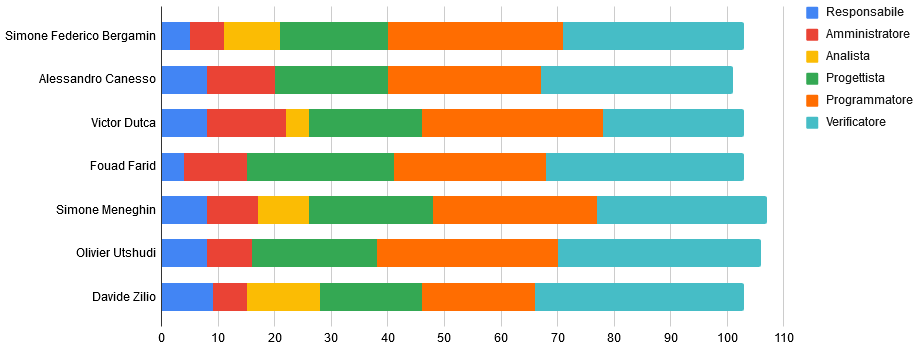
\includegraphics[scale=0.60]{img/grafici/tabella_tot_no_analisi.png}
\caption{Istogramma della ripartizione delle ore totali per ruolo con investimento}
\end{figure}

\paragraph{Prospetto economico} \mbox{} \\ \mbox{} \\
Il costo totale senza investimento è riportato nella seguente tabella:

%tabella costi
\begin{table}[H]
\centering\renewcommand{\arraystretch}{1.5}
\caption{Costi totali senza investimento}
\vspace{0.2cm}
\begin{tabular}{ c | c | c  }
\rowcolor{redafk}
\textcolor{white}{\textbf{Ruolo}} & \textcolor{white}{\textbf{Ore}} & 
\textcolor{white}{\textbf{Costo}}  \\
Responsabile & 50 & 1500€ \\
Amministratore & 66 & 1320€ \\
Analista & 36 & 900€ \\
Progettista	& 147 & 3234€ \\
Programmatore & 198 & 2970€  \\
Verificatore & 229 & 3435€  \\
\rowcolor{lastrowcolor}
\textbf{Totale} & \textbf{729} & \textbf{13359€}  \\
\end{tabular}
\end{table}

I dati ottenuti si possono riassumere nel seguente areogramma:
\begin{figure}[H]
\centering
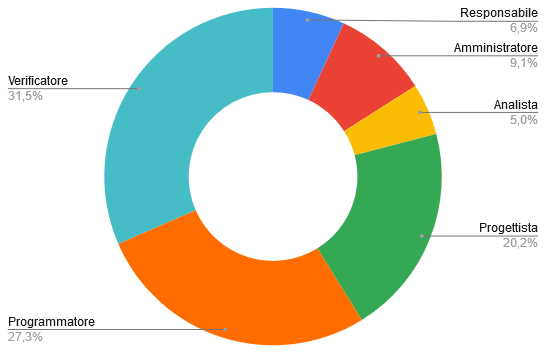
\includegraphics[scale=0.60]{img/grafici/torta_tot_no_analisi.png}
\caption{Areogramma della ripartizione dei costi totali per ruolo senza investimento}
\end{figure}

\subsection{Conclusioni}
Il costo totale preventivato per il progetto è 13.359,00€